\documentclass[12pt,a4paper]{article}
\usepackage[utf8]{inputenc}
\usepackage[T1]{fontenc}
\usepackage[spanish]{babel}
\usepackage{geometry}
\usepackage{setspace}
\usepackage{booktabs}
\usepackage{graphicx}
\usepackage{float}
\usepackage{caption}
\usepackage{longtable}
\usepackage{tabularx}
\usepackage{adjustbox}
\usepackage{hyperref}
\usepackage{titlesec}
\usepackage{tocloft}
\usepackage{array}

\geometry{margin=2.54cm}
\onehalfspacing
\setlength{\parindent}{1.27cm}
\setlength{\parskip}{0pt}
\captionsetup{font=small, labelfont=bf}
\renewcommand{\tablename}{Tabla}
\renewcommand{\figurename}{Figura}
\hypersetup{colorlinks=true,linkcolor=black,urlcolor=black,citecolor=black}
\titleformat{\section}{\normalfont\bfseries\fontsize{12}{14}\selectfont}{\thesection.}{0.5em}{}
\titleformat{\subsection}{\normalfont\bfseries\fontsize{12}{14}\selectfont}{\thesubsection.}{0.5em}{}

\newcommand{\apatableinput}[1]{
\begin{table}[H]
\centering
\begin{adjustbox}{max width=\textwidth}
\input{#1}
\end{adjustbox}
\end{table}
}

\begin{document}

\begin{titlepage}
\centering
{\Large Universidad EAN\par}
\vspace{1.2cm}
{\large Seminario de Investigación\par}
\vspace{1.2cm}
{\Large\bfseries Informe técnico avanzado: calidad de condiciones de estudio en bibliotecas públicas de Bogotá\par}
\vspace{1.6cm}
{\large Alejandro Roa Aparicio\par}
{\large Alisson Dayana Navarro Rodríguez\par}
\vspace{1.2cm}
{\large Profesor: Diego Armando García García\par}
\vfill
{\large 2026\par}
\end{titlepage}

\pagenumbering{roman}
\setcounter{page}{1}

\section*{Resumen}
Este informe presenta una evaluación estadística avanzada de iluminación, ruido y conectividad WiFi en bibliotecas públicas de Bogotá. Además de métricas descriptivas, se incorporan intervalos de confianza, tamaño del efecto para pruebas no paramétricas, comparaciones post-hoc ajustadas, análisis de valores atípicos y modelos de regresión robusta. El objetivo es generar evidencia técnicamente sólida para priorizar intervenciones de infraestructura y gestión operativa desde una perspectiva de experiencia de usuario y política pública urbana.

\newpage
\tableofcontents
\newpage
\listoftables
\newpage
\listoffigures
\newpage

\pagenumbering{arabic}
\setcounter{page}{1}

\section{Introducción}
La calidad ambiental de espacios bibliotecarios condiciona la eficacia del estudio, la permanencia de usuarios y la equidad en acceso a servicios públicos de aprendizaje. En contextos urbanos densos, la calidad de iluminación, confort acústico y conectividad digital debe abordarse como un sistema integrado de desempeño, no como variables aisladas. Este documento eleva el análisis previo hacia un estándar técnico cercano a informe publicable, incorporando inferencia estadística y criterios de priorización estratégica.

\section{Metodología}
\subsection{Datos y preprocesamiento}
Se consolidaron todos los archivos de la carpeta \texttt{Datos/}, normalizando variaciones de encabezados y hojas. Se depuraron registros vacíos y se estandarizaron variables de interés (\textit{Lux\_promedio}, \textit{dBA\_prom}, \textit{Bajada\_Mediana}, ocupación y metadatos temporales).

\subsection{Criterios de cumplimiento}
Se definieron umbrales operativos:
\begin{itemize}
    \item Iluminación: 500 lux (lectura), 200 lux (estanterías), 300 lux (circulación/general).
    \item Ruido: $dBA\_prom \leq 40$.
    \item WiFi: bajada mediana $\geq 10$ Mbps.
\end{itemize}
Se estimaron dos índices: (a) índice compuesto simple (promedio de tres cumplimientos), y (b) índice ponderado propuesto (40\% luz, 40\% ruido, 20\% WiFi).

\subsection{Métodos estadísticos avanzados}
El análisis incluyó:
\begin{itemize}
    \item Intervalos de confianza bootstrap al 95\% para métricas globales.
    \item Prueba de Kruskal--Wallis entre bibliotecas con tamaño del efecto ($\epsilon^2$).
    \item Comparaciones post-hoc (Mann--Whitney) con ajuste de Holm y tamaño del efecto (Cliff's Delta).
    \item Detección de outliers por criterio IQR.
    \item Modelos OLS con errores robustos (HC3) para explorar relación de ocupación/franja con ruido y WiFi.
\end{itemize}

\section{Resultados}
\subsection{Caracterización general}
\apatableinput{tablas/resumen_general.tex}
\apatableinput{tablas/intervalos_confianza.tex}
\noindentEste estudio consolidó 1420 registros válidos de 17 bibliotecas y 13 localidades. El cumplimiento global fue de 39.2\% para iluminación, 13.5\% para ruido y 78.2\% para WiFi. En términos de desempeño integral, el índice simple promedio fue 43.6/100 y el índice ponderado propuesto fue 36.7/100.

Las bibliotecas de mayor desempeño ponderado fueron: Biblioteca Luis Angel Arango (86.4); Luis Ángel Arango (77.8); Biblioteca Casa Gómez Campuzano (64.0). Las de menor desempeño fueron: Biblioteca Pública del Deporte - CEFE Chapinero (20.0); Biblioteca Pública Virgilio Barco (18.6); Gabriel Garcia Marquez - Tunal (16.1).


\begin{figure}[H]
\centering
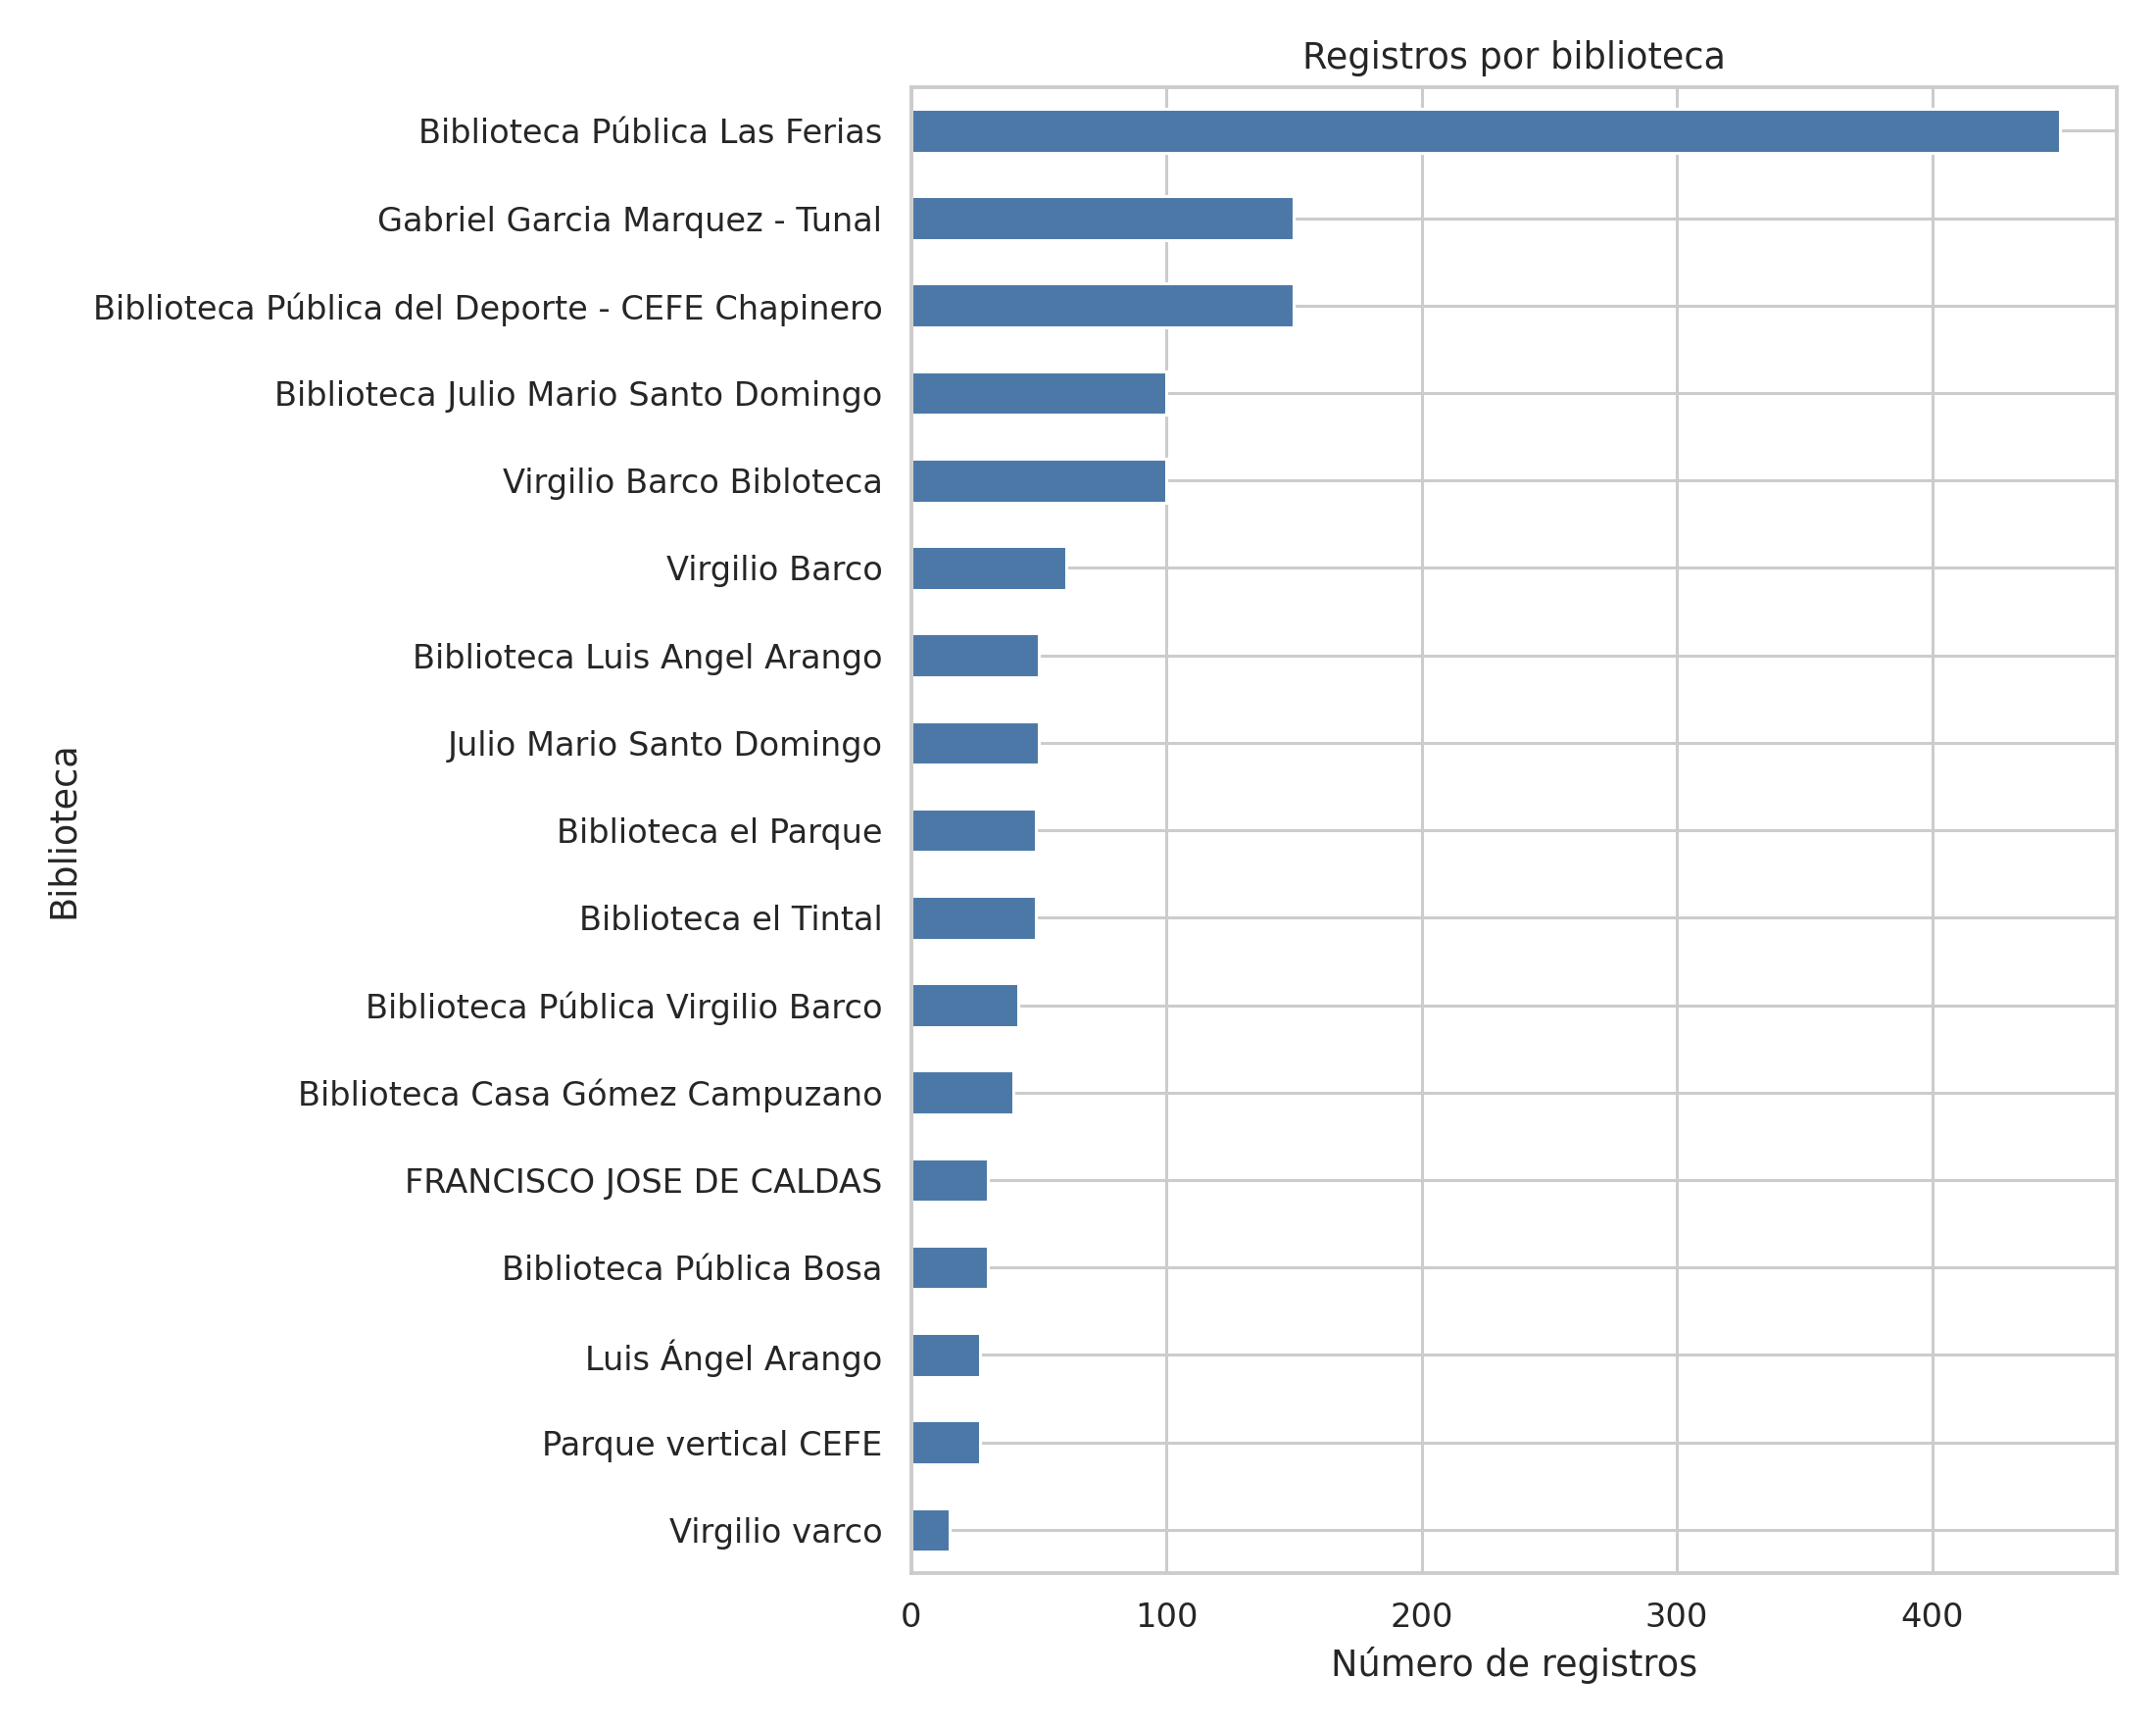
\includegraphics[width=0.88\textwidth]{figuras/registros_por_biblioteca.png}
\caption{Distribución del tamaño muestral por biblioteca.}
\end{figure}
\noindent\textbf{Interpretación crítica.} La heterogeneidad de tamaño muestral entre bibliotecas condiciona la precisión de estimación. Por ello, los resultados se interpretan junto con dispersión, intervalos y efecto, evitando inferencias basadas únicamente en medias puntuales.

\subsection{Análisis comparativo por biblioteca}
\apatableinput{tablas/resumen_biblioteca.tex}
\apatableinput{tablas/cumplimiento.tex}
\noindentLas pruebas de Kruskal--Wallis evidenciaron diferencias estadísticamente significativas entre bibliotecas en los tres ejes analizados, con los siguientes resultados: Lux\_promedio (H=583.10, p=0.0000, epsilon-cuadrado=0.413, efecto grande); dBA\_prom (H=544.29, p=0.0000, epsilon-cuadrado=0.377, efecto grande); Bajada\_Mediana (H=818.01, p=0.0000, epsilon-cuadrado=0.572, efecto grande). Reportar p muy pequeño (aprox. 0.0000) no implica efecto infinito; por ello se complementó con tamaño del efecto, mostrando que las diferencias tienen magnitud sustantiva y no solo significancia por tamaño muestral.

En el análisis post-hoc (Mann--Whitney con ajuste de Holm) se identificaron contrastes puntuales robustos entre pares de bibliotecas. Los principales fueron: Lux\_promedio: Biblioteca Pública Las Ferias vs Virgilio Barco Bibloteca (p-aj=0.0000, delta=-0.996); Lux\_promedio: Biblioteca Pública del Deporte - CEFE Chapinero vs Virgilio Barco Bibloteca (p-aj=0.0000, delta=-1.000); Lux\_promedio: Gabriel Garcia Marquez - Tunal vs Virgilio Barco Bibloteca (p-aj=0.0000, delta=-0.991); Lux\_promedio: Biblioteca Julio Mario Santo Domingo vs Virgilio Barco Bibloteca (p-aj=0.0000, delta=-0.987); Lux\_promedio: Biblioteca Luis Angel Arango vs Biblioteca Pública del Deporte - CEFE Chapinero (p-aj=0.0000, delta=1.000); Lux\_promedio: Biblioteca Pública del Deporte - CEFE Chapinero vs Julio Mario Santo Domingo (p-aj=0.0000, delta=-1.000). Esto respalda que la heterogeneidad no es uniforme, sino concentrada en comparaciones específicas de sedes.

El análisis de valores atípicos mostró la siguiente incidencia: Lux\_promedio: 10.9%; dBA\_prom: 3.5%; Bajada\_Mediana: 12.0%. Este hallazgo sugiere episodios operativos extremos (picos de ruido o variabilidad de red) que deben gestionarse con estrategias de monitoreo continuo, no solo con promedios.

En modelos explicativos robustos, la ocupación mostró asociación positiva con ruido (coef=-0.361, p=0.0000), mientras que su relación con velocidad de bajada fue menor (coef=0.780, p=0.0003). En términos prácticos, la presión de usuarios parece impactar más directamente el confort acústico que la capacidad de red promedio, lo que sugiere priorizar rediseño espacial y control de carga acústica en franjas críticas.


\begin{figure}[H]
\centering
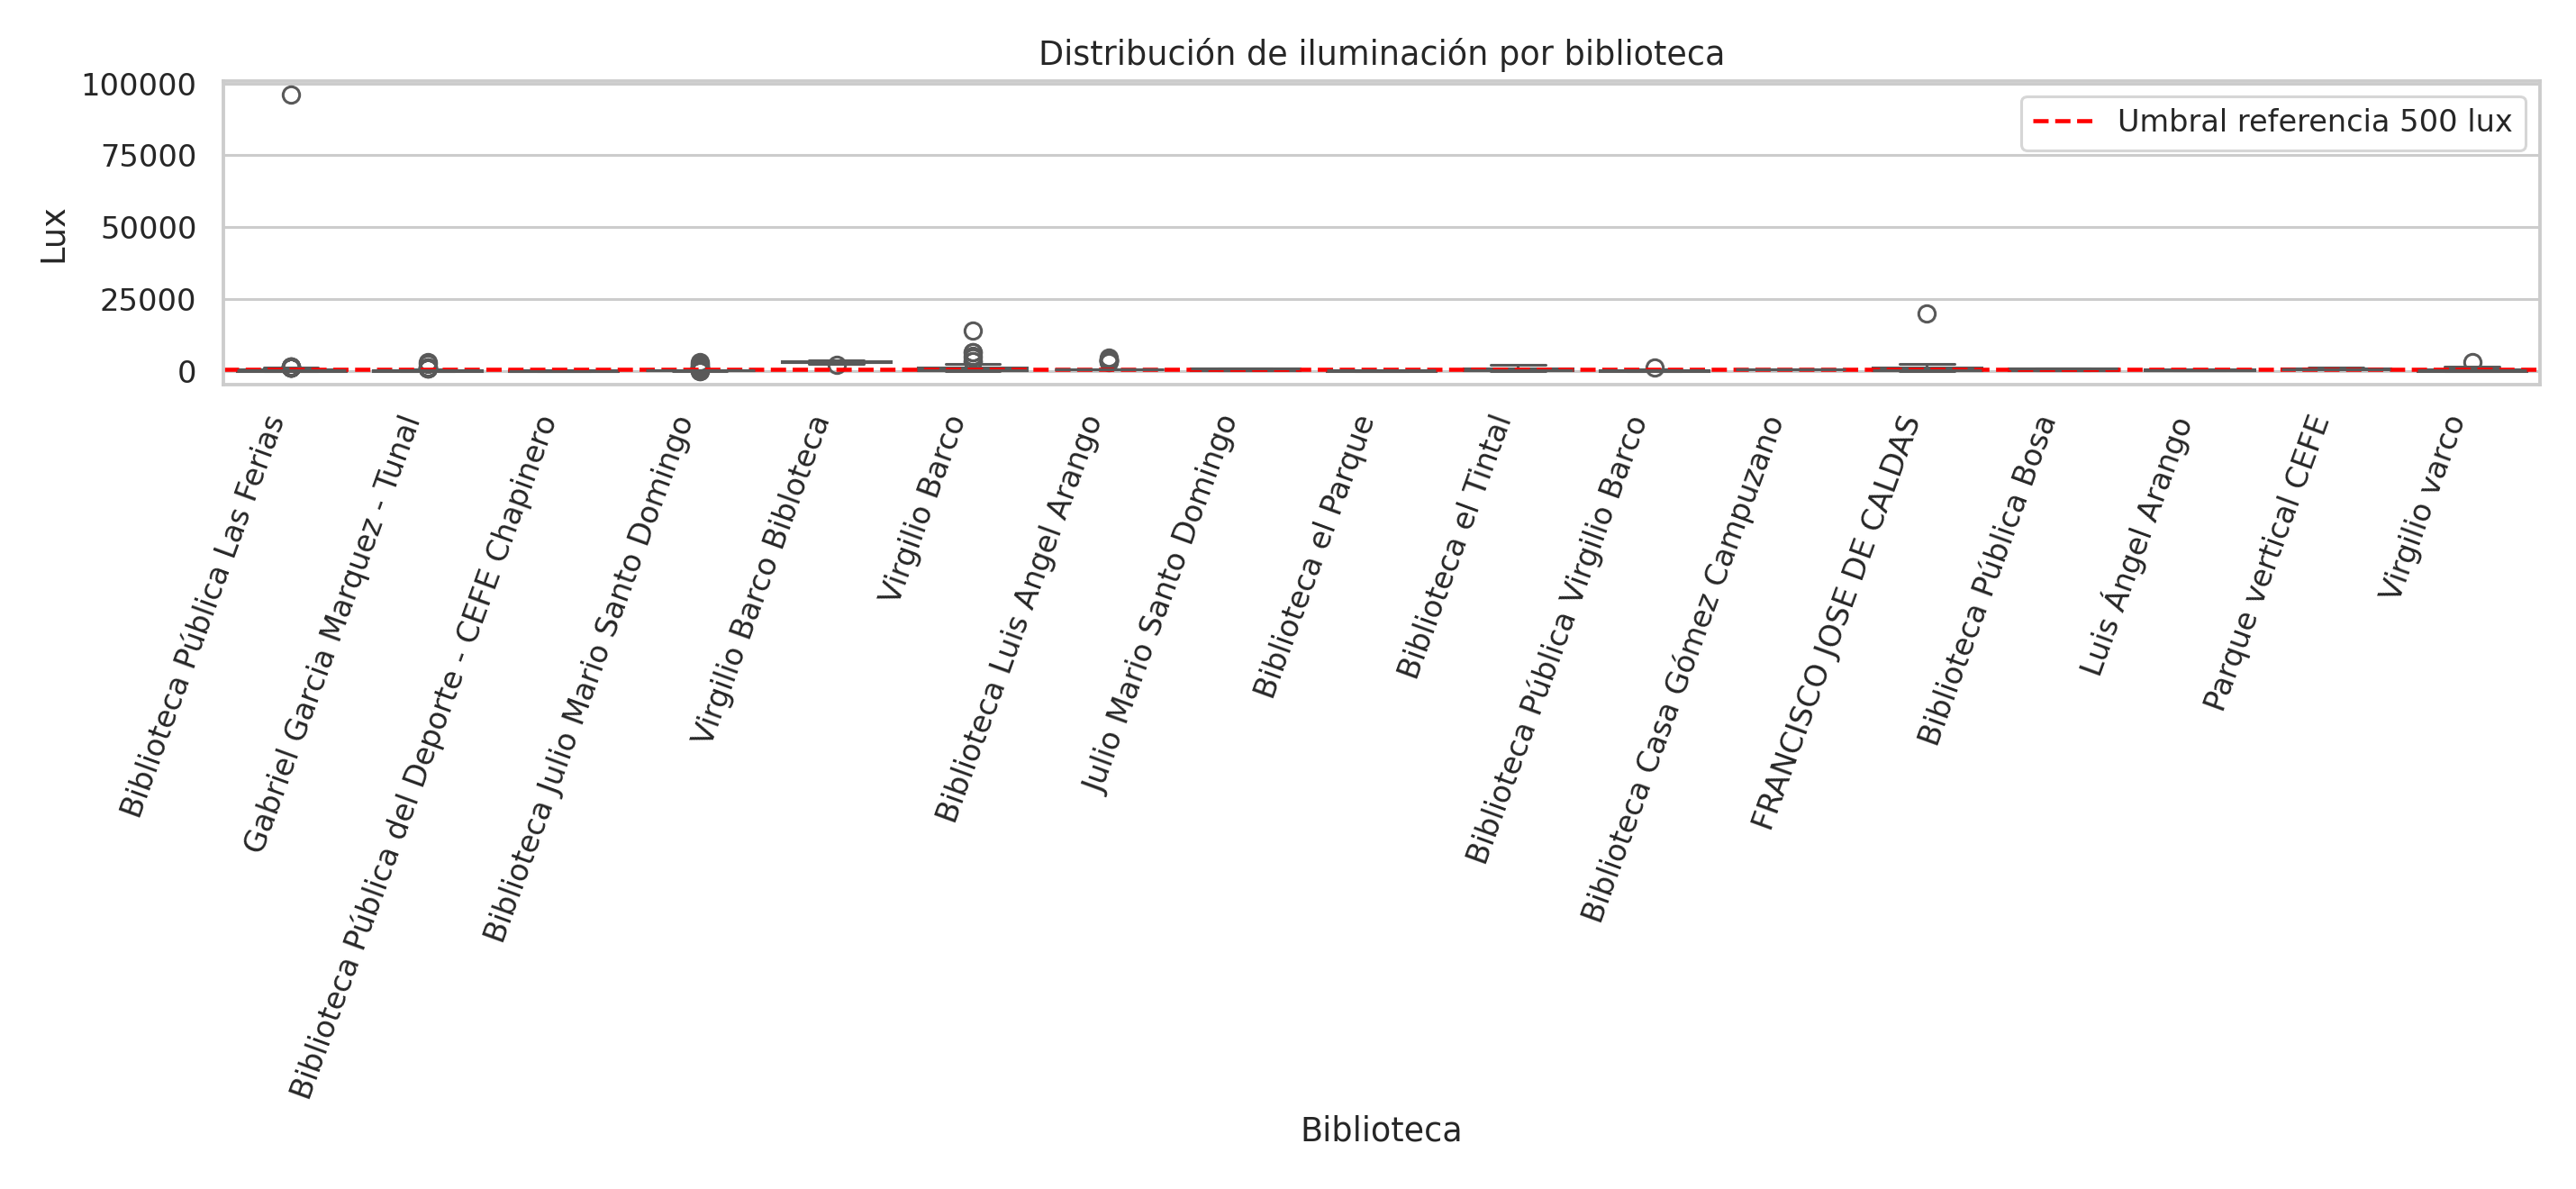
\includegraphics[width=\textwidth]{figuras/box_lux_biblioteca.png}
\caption{Distribución de iluminación por biblioteca (lux).}
\end{figure}
\noindent\textbf{Interpretación crítica.} La amplitud intercuartílica y la presencia de extremos muestran que la calidad lumínica es altamente variable entre sedes. Este patrón sugiere diferencias estructurales de diseño interior y mantenimiento que no se corrigen con intervenciones homogéneas.

\begin{figure}[H]
\centering
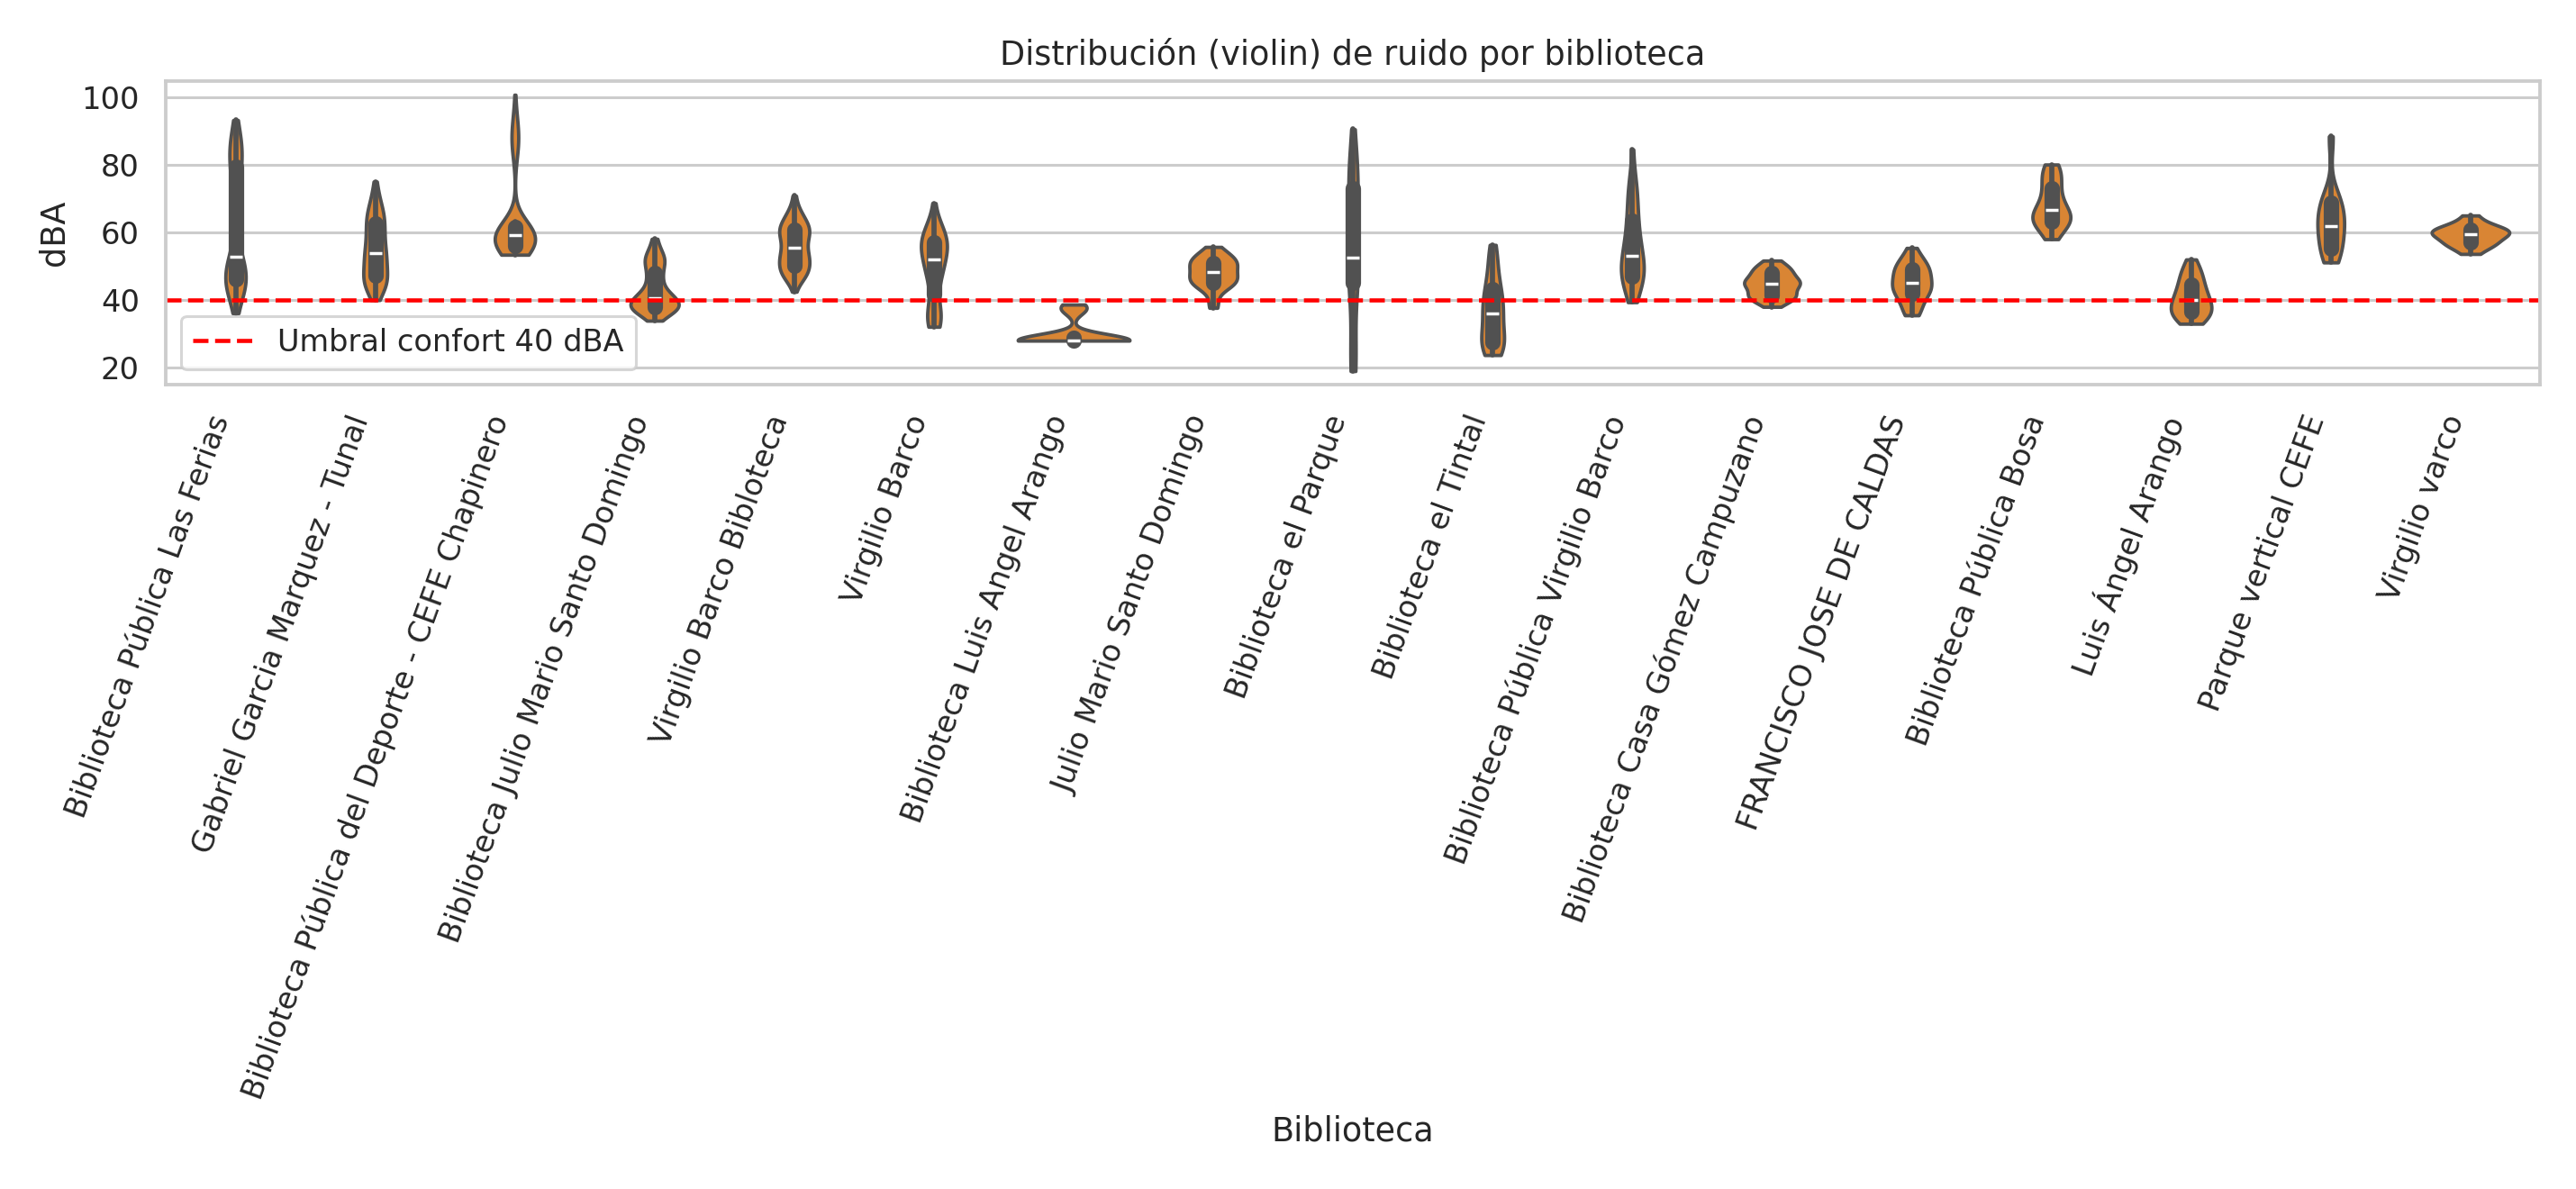
\includegraphics[width=\textwidth]{figuras/violin_ruido_biblioteca.png}
\caption{Distribución de ruido por biblioteca (dBA) mediante violin plot.}
\end{figure}
\noindent\textbf{Interpretación crítica.} El violin plot revela multimodalidad en varias sedes, compatible con alternancia de periodos de baja y alta perturbación acústica. Esta evidencia es más informativa que un boxplot simple para identificar inestabilidad operativa.

\begin{figure}[H]
\centering
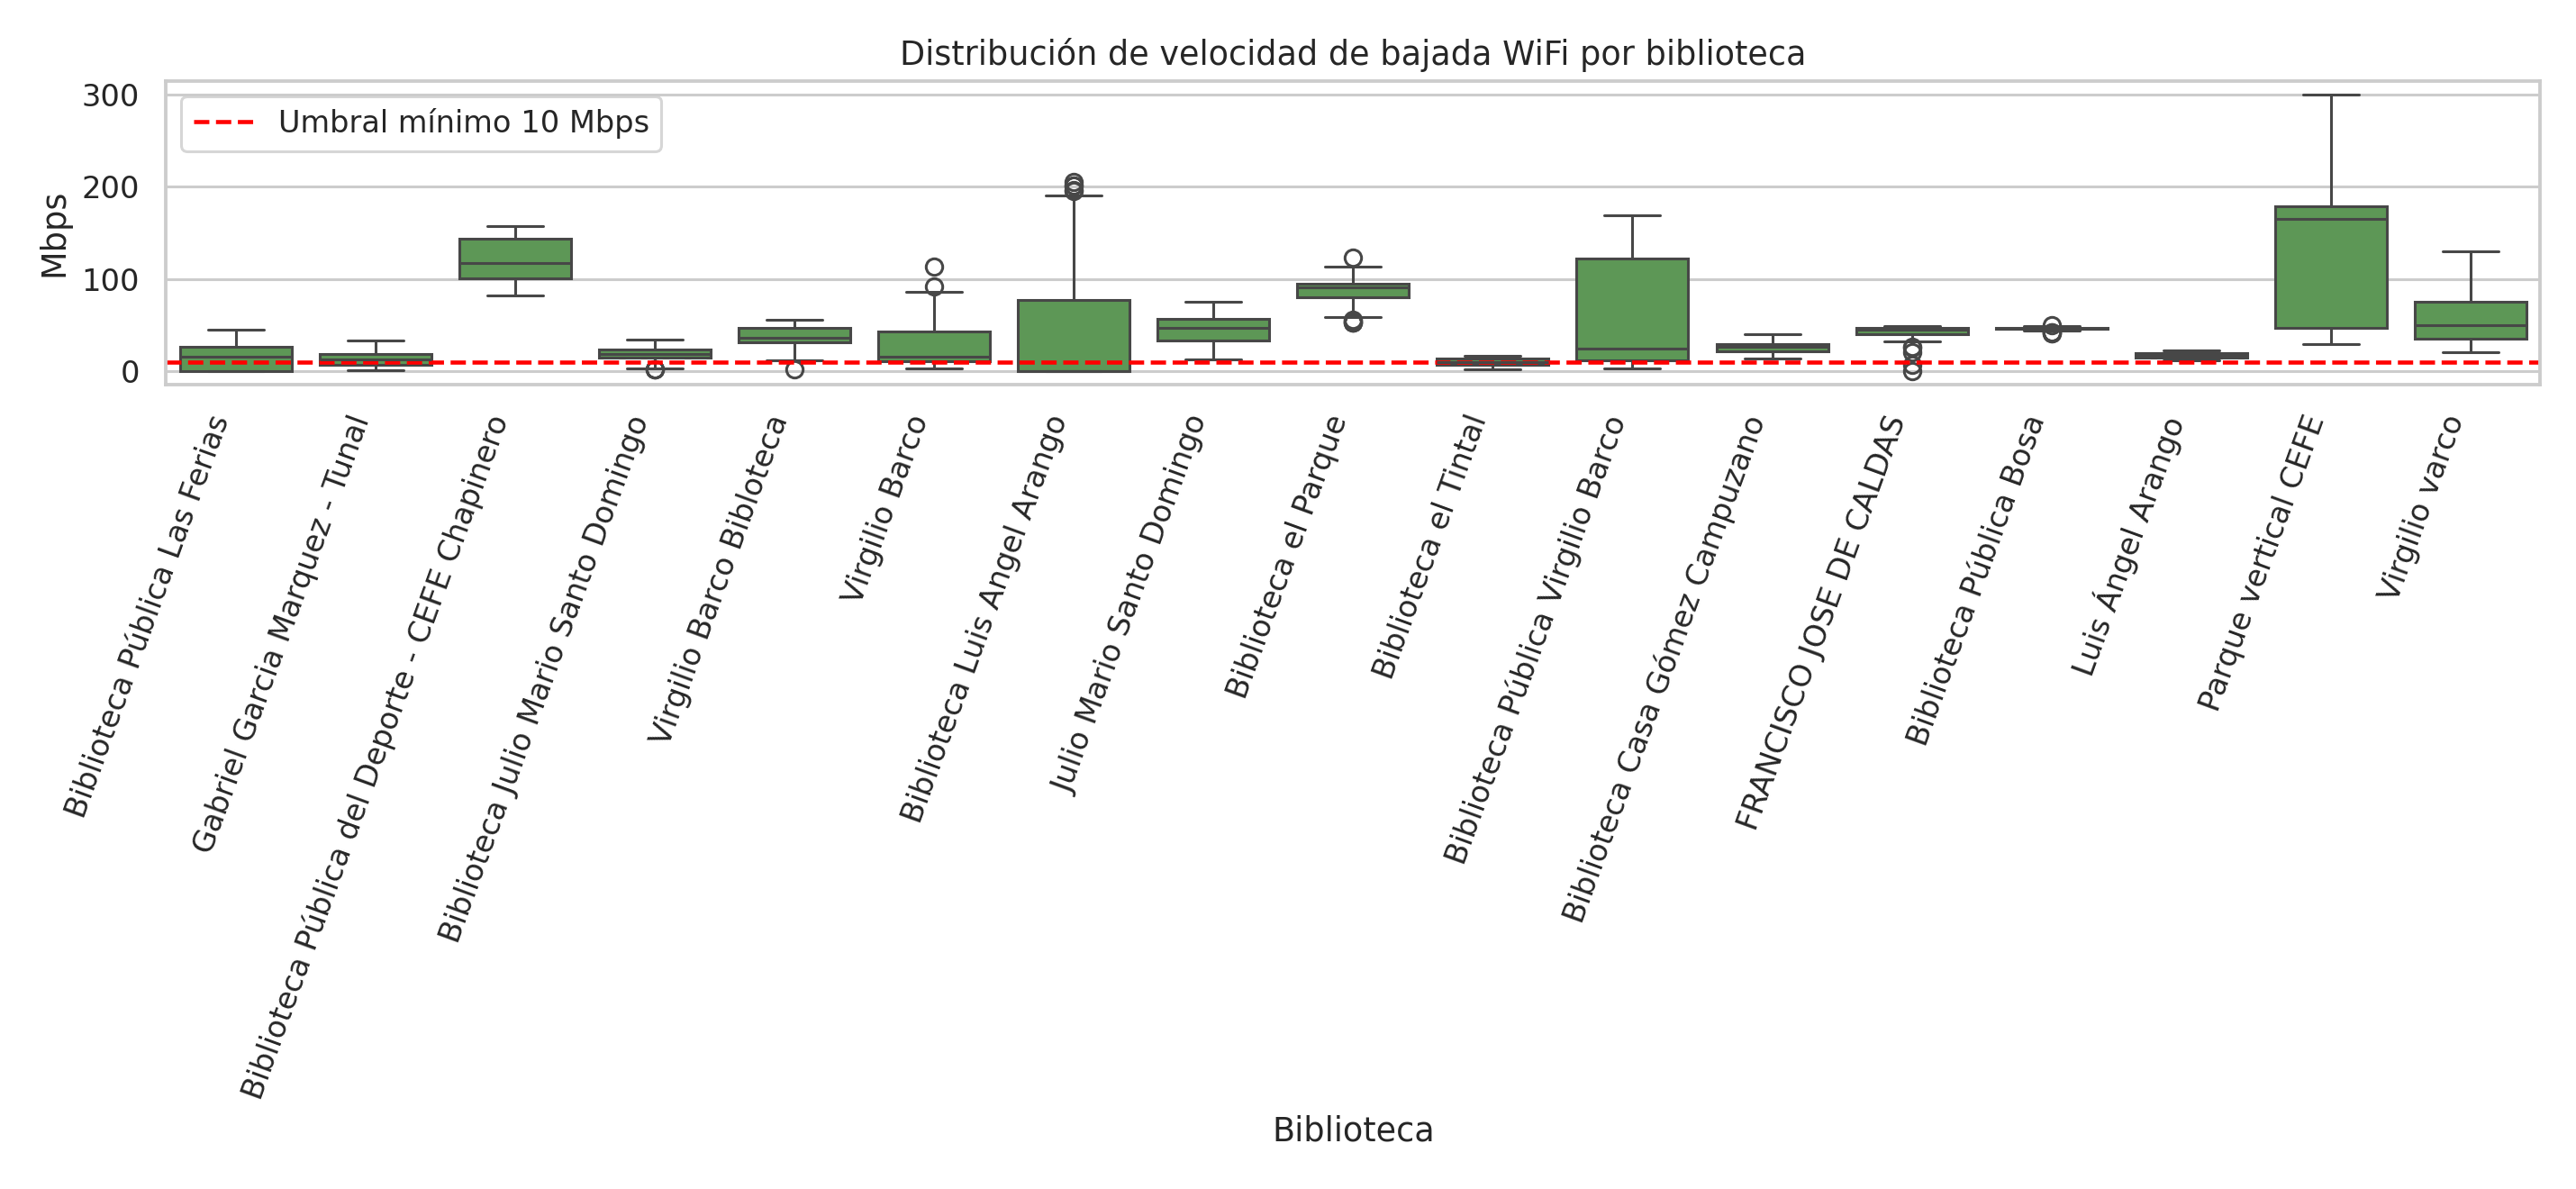
\includegraphics[width=\textwidth]{figuras/box_wifi_biblioteca.png}
\caption{Distribución de velocidad de bajada WiFi por biblioteca (Mbps).}
\end{figure}
\noindent\textbf{Interpretación crítica.} Aunque múltiples sedes superan el umbral mínimo, la dispersión interna evidencia desigualdad de experiencia digital. Para usuarios, esto se traduce en confiabilidad heterogénea del servicio en tareas académicas intensivas.

\subsection{Cumplimiento, priorización e índice mejorado}
\begin{figure}[H]
\centering
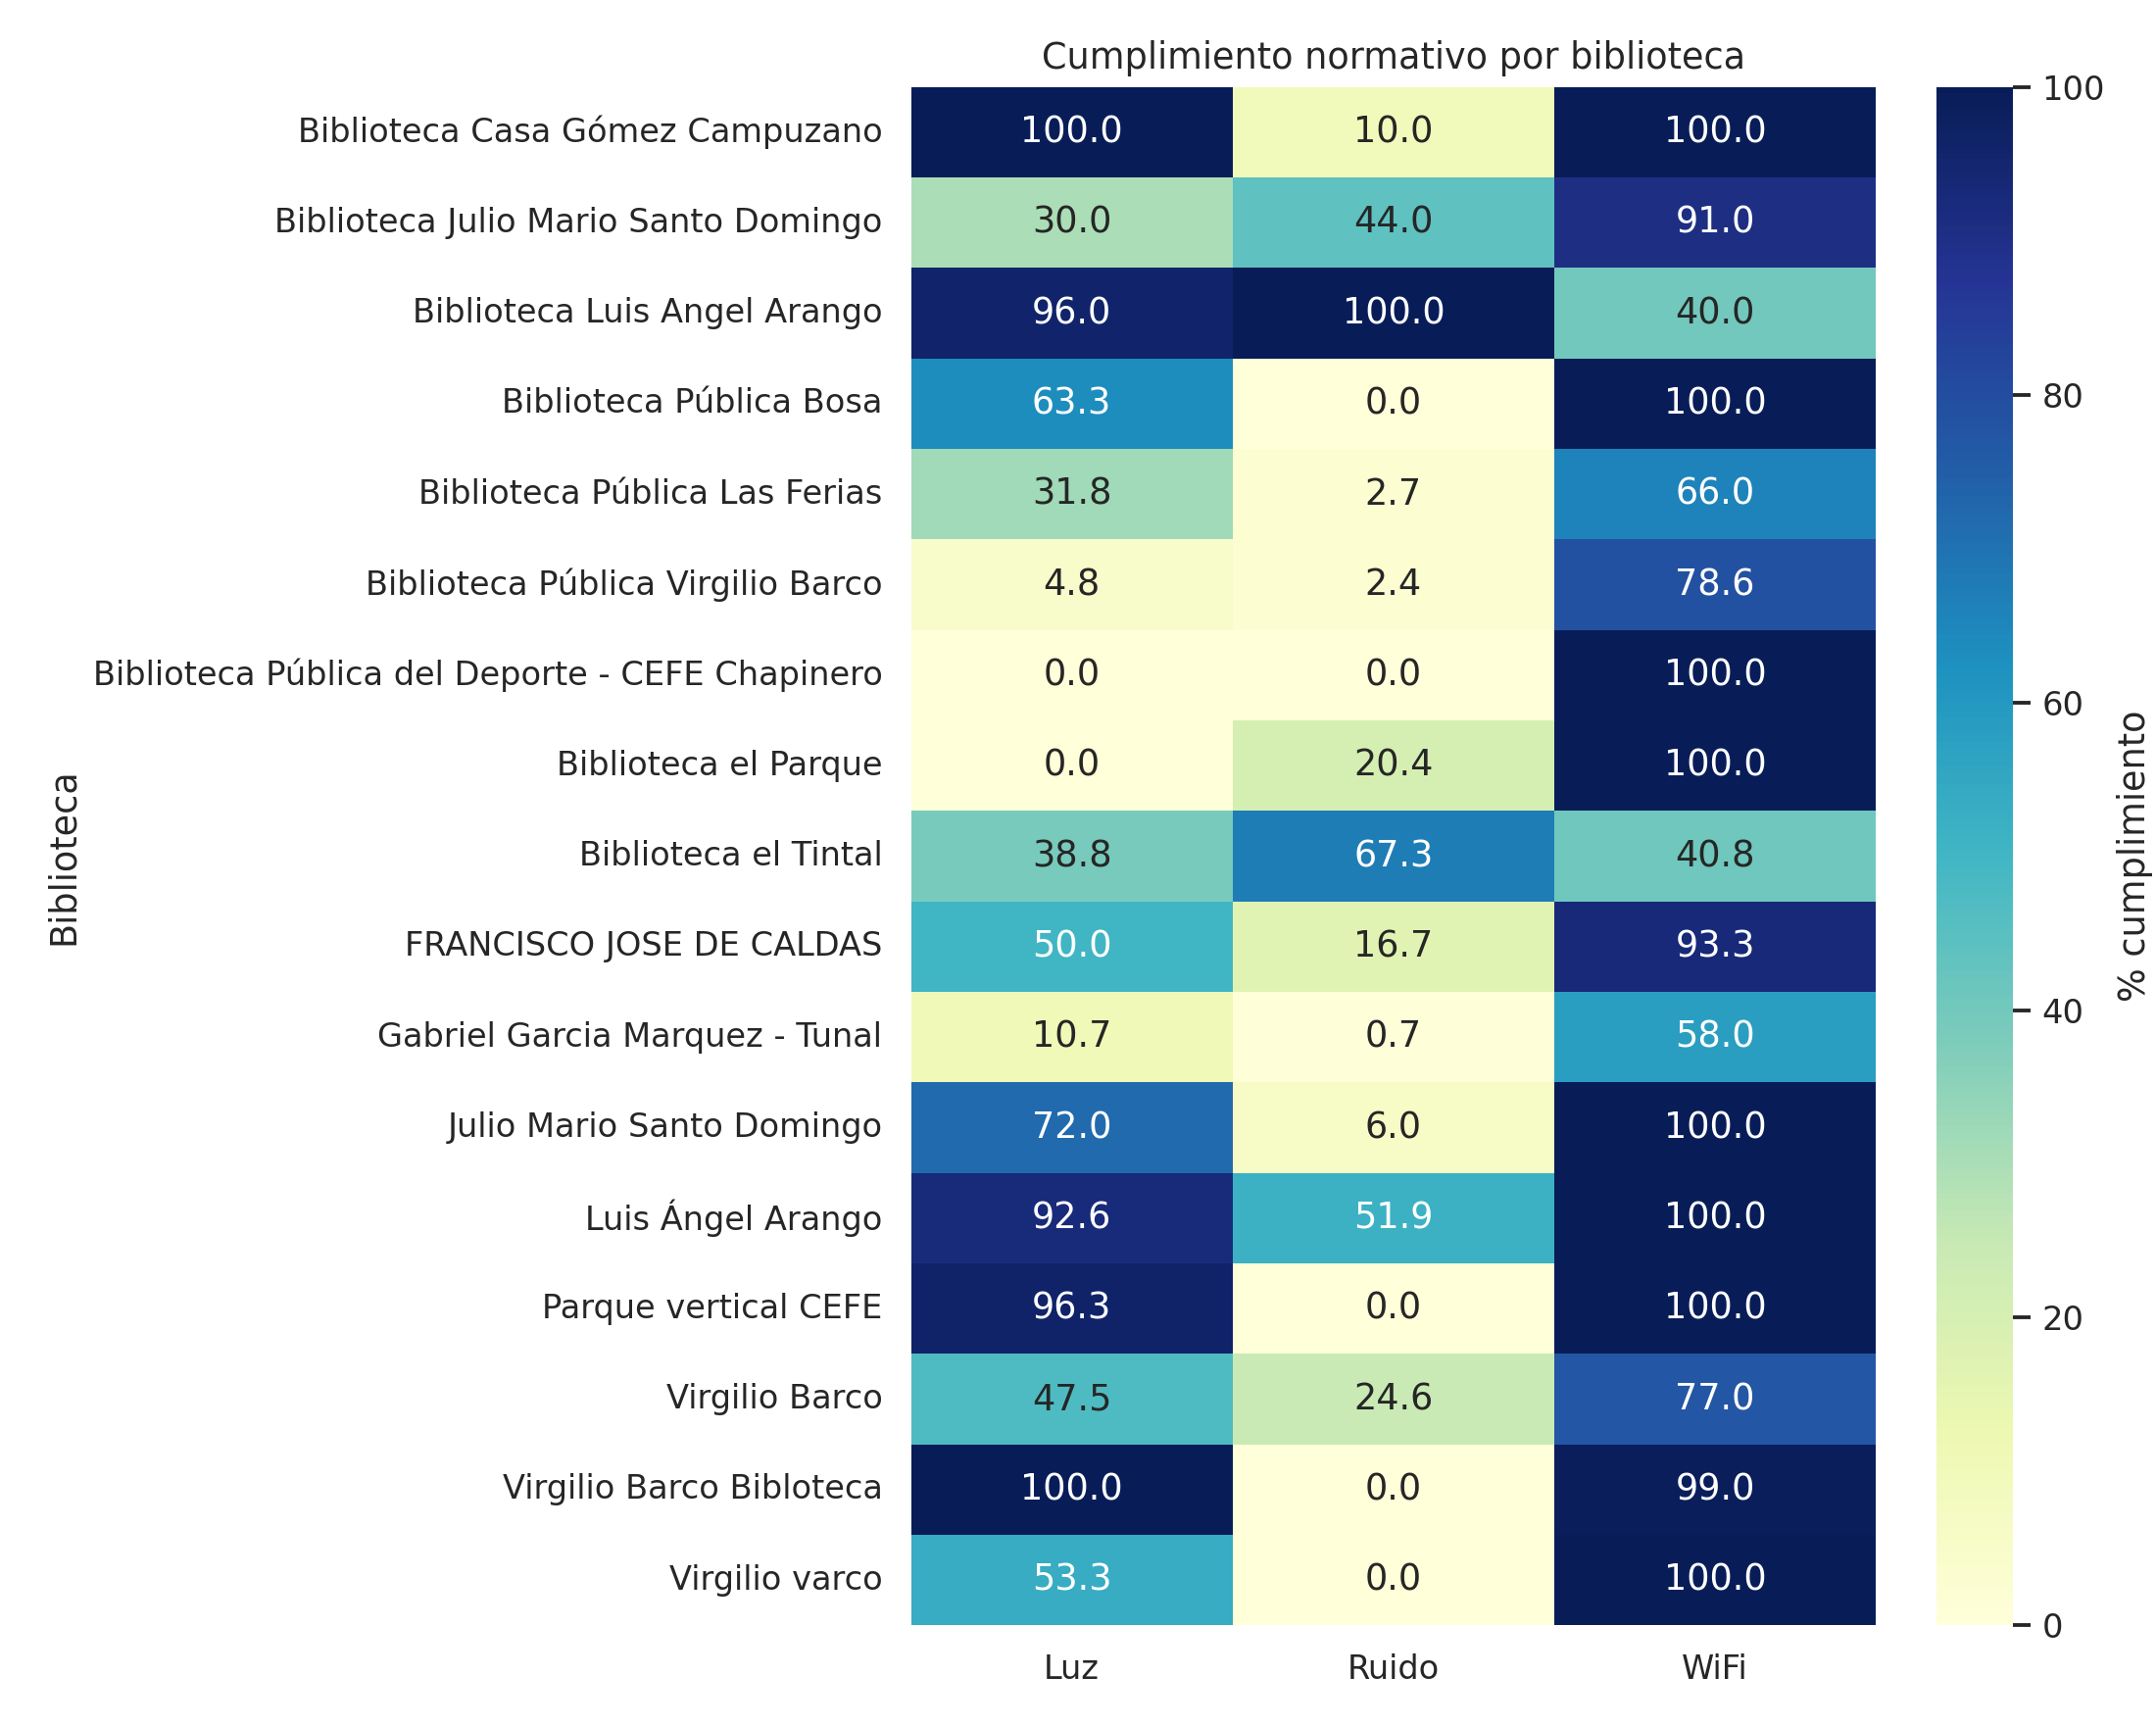
\includegraphics[width=0.90\textwidth]{figuras/heatmap_cumplimiento.png}
\caption{Matriz de cumplimiento por criterio y biblioteca.}
\end{figure}
\noindent\textbf{Interpretación crítica.} El patrón cruzado de cumplimiento muestra que ninguna dimensión explica por sí sola el desempeño total. Esto justifica la evaluación multicriterio y la priorización por perfil de brecha, no solo por promedio general.

\begin{figure}[H]
\centering
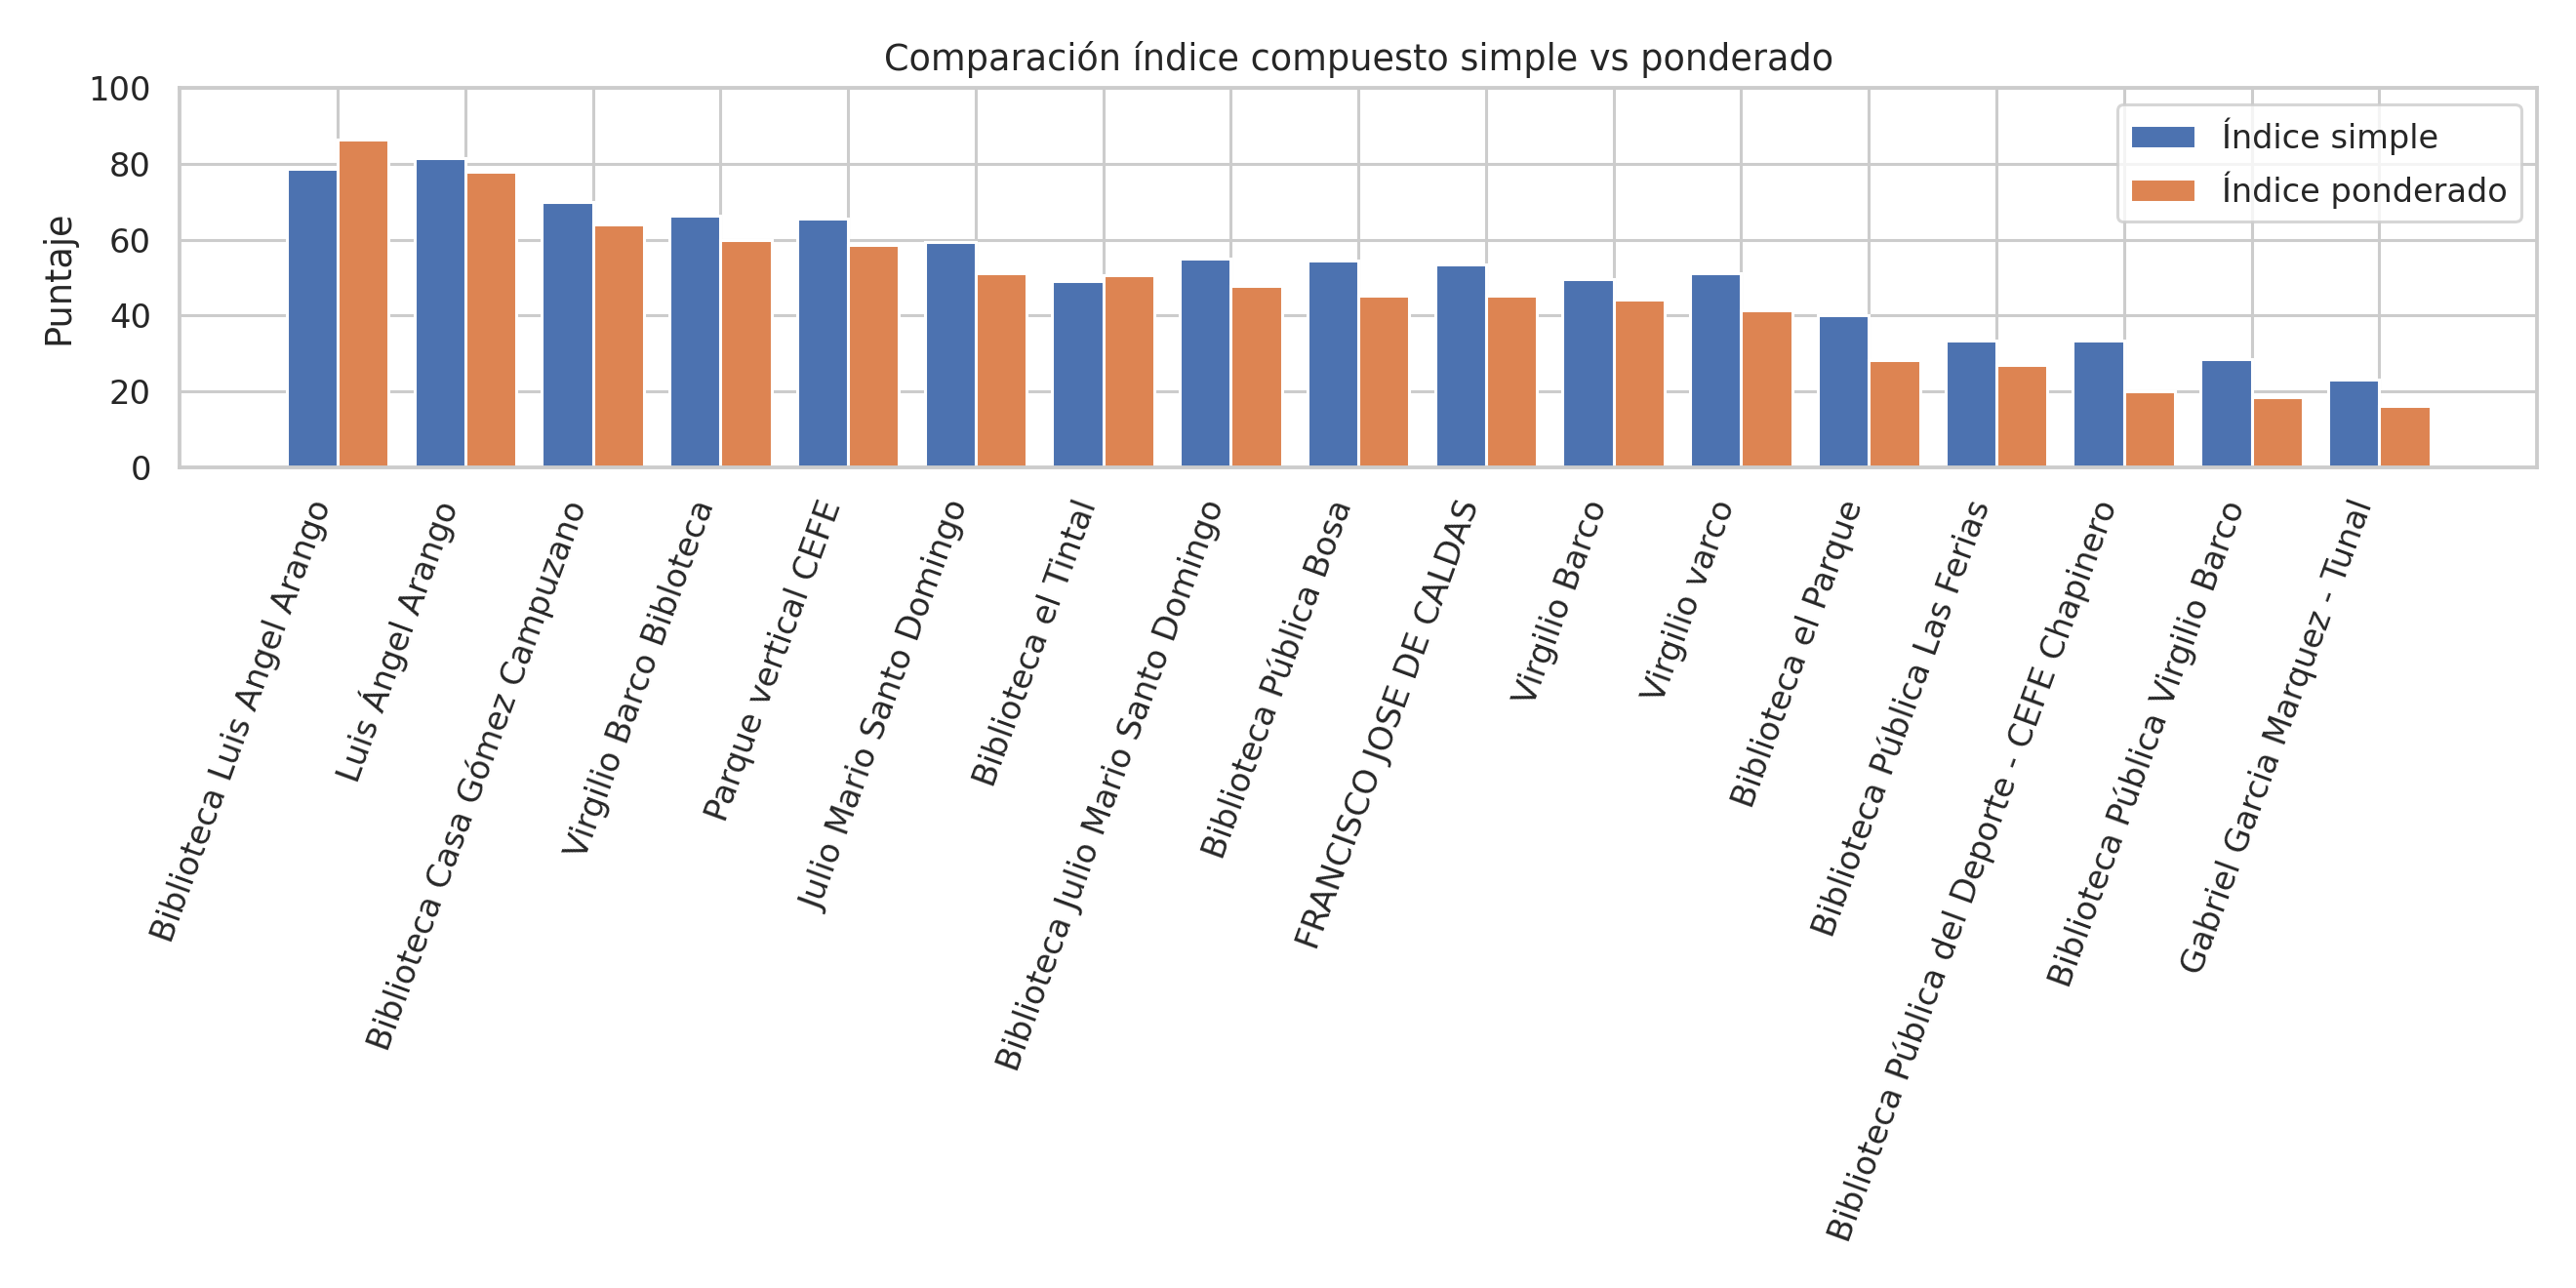
\includegraphics[width=\textwidth]{figuras/indice_simple_vs_ponderado.png}
\caption{Comparación entre índice simple y ponderado por biblioteca.}
\end{figure}
\noindent\textbf{Interpretación crítica.} El cambio de ranking entre índices confirma que el promedio simple puede infraestimar bibliotecas con déficits en confort ambiental. El índice ponderado mejora la validez práctica cuando la política de mejora prioriza permanencia y concentración en sala.

\noindentEl índice compuesto actual (promedio simple) asume igual importancia entre iluminación, ruido y WiFi. Esta suposición facilita interpretación, pero puede subestimar dimensiones de mayor impacto en experiencia de estudio. Como mejora, se propone un índice ponderado: 40\% iluminación, 40\% ruido y 20\% WiFi. Esta ponderación prioriza condiciones de confort cognitivo y permanencia en sala.

Adicionalmente, se recomienda explorar ponderaciones basadas en evidencia empírica (por ejemplo, análisis factorial, preferencias de usuario o validación con desempeño académico), con evaluación de robustez por sensibilidad de pesos.

\apatableinput{tablas/prioridades.tex}

\subsection{Inferencia estadística y robustez}
\apatableinput{tablas/efecto_kruskal.tex}
\apatableinput{tablas/posthoc_significativos.tex}
\apatableinput{tablas/outliers_resumen.tex}
\noindent\textbf{Interpretación crítica.} La convergencia entre significancia estadística, tamaño del efecto y contrastes post-hoc respalda que las diferencias observadas son sustantivas y operativamente relevantes. El componente de outliers sugiere que la gestión de eventos extremos debe integrarse al diseño de política, no tratarse como ruido analítico.

\subsection{Modelos explicativos}
\apatableinput{tablas/regresion_ruido.tex}
\apatableinput{tablas/regresion_wifi.tex}

\begin{figure}[H]
\centering
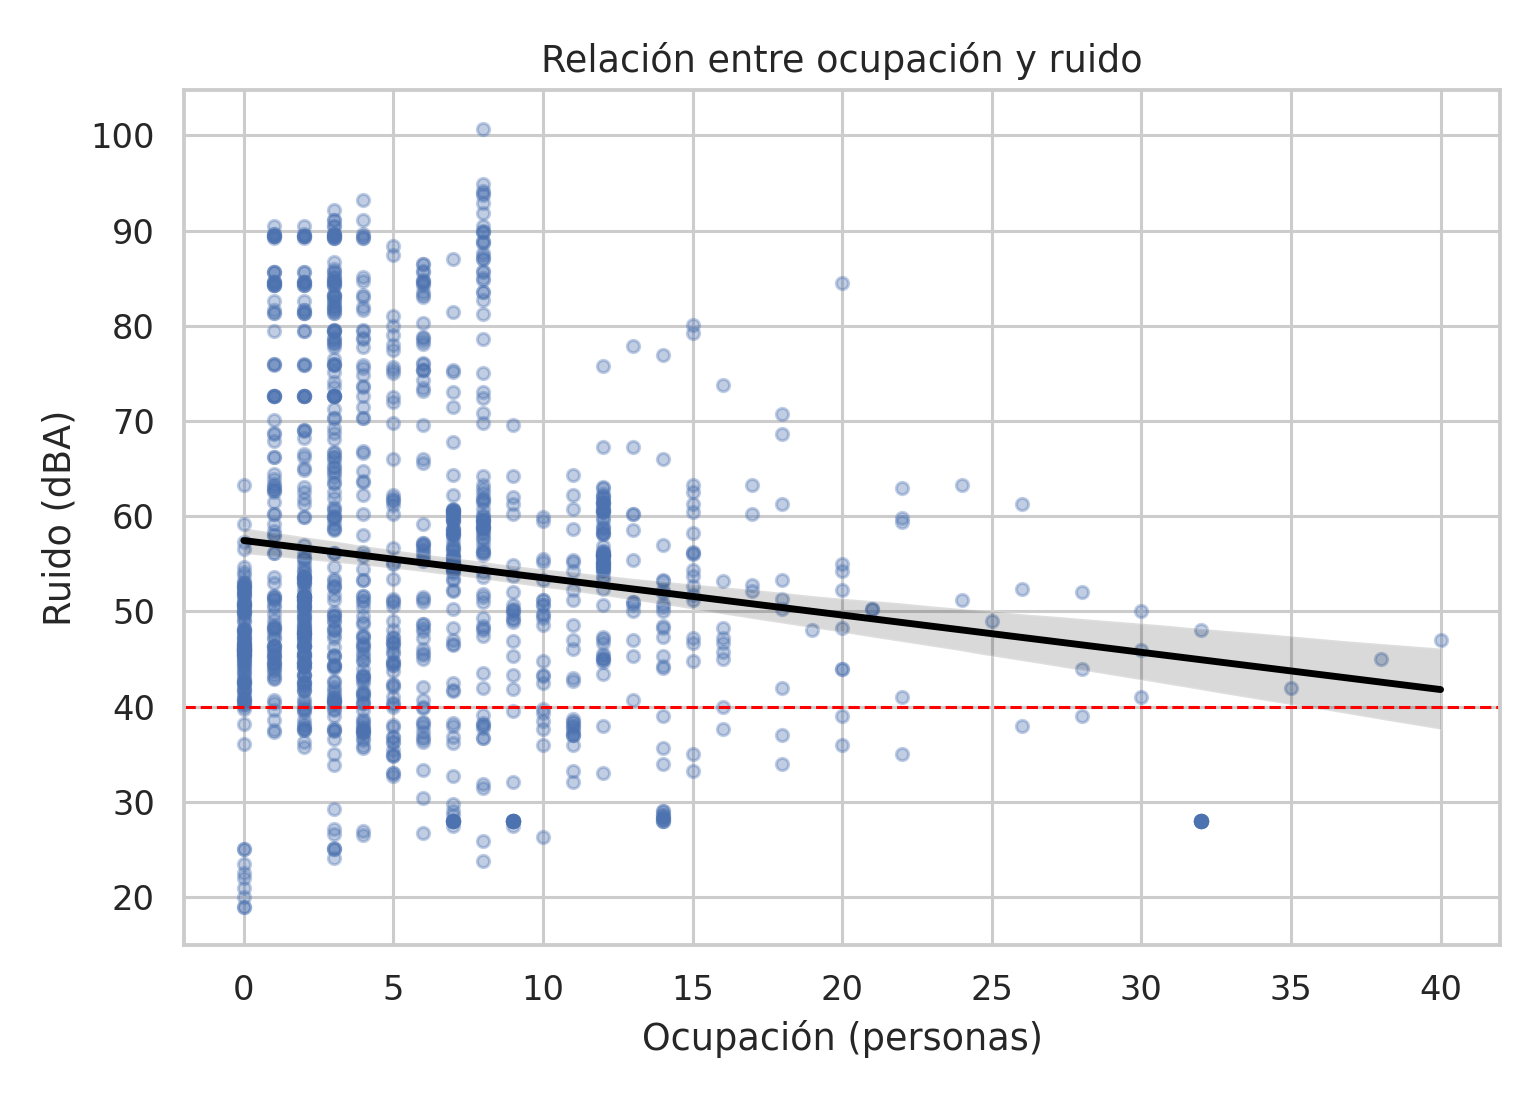
\includegraphics[width=0.8\textwidth]{figuras/scatter_ocupacion_ruido.png}
\caption{Relación entre ocupación y ruido (ajuste lineal).}
\end{figure}
\noindent\textbf{Interpretación crítica.} La pendiente positiva respalda la hipótesis de carga acústica por demanda. En términos de gestión, la ocupación debe tratarse como variable de control operativo para proteger condiciones de estudio.

\begin{figure}[H]
\centering
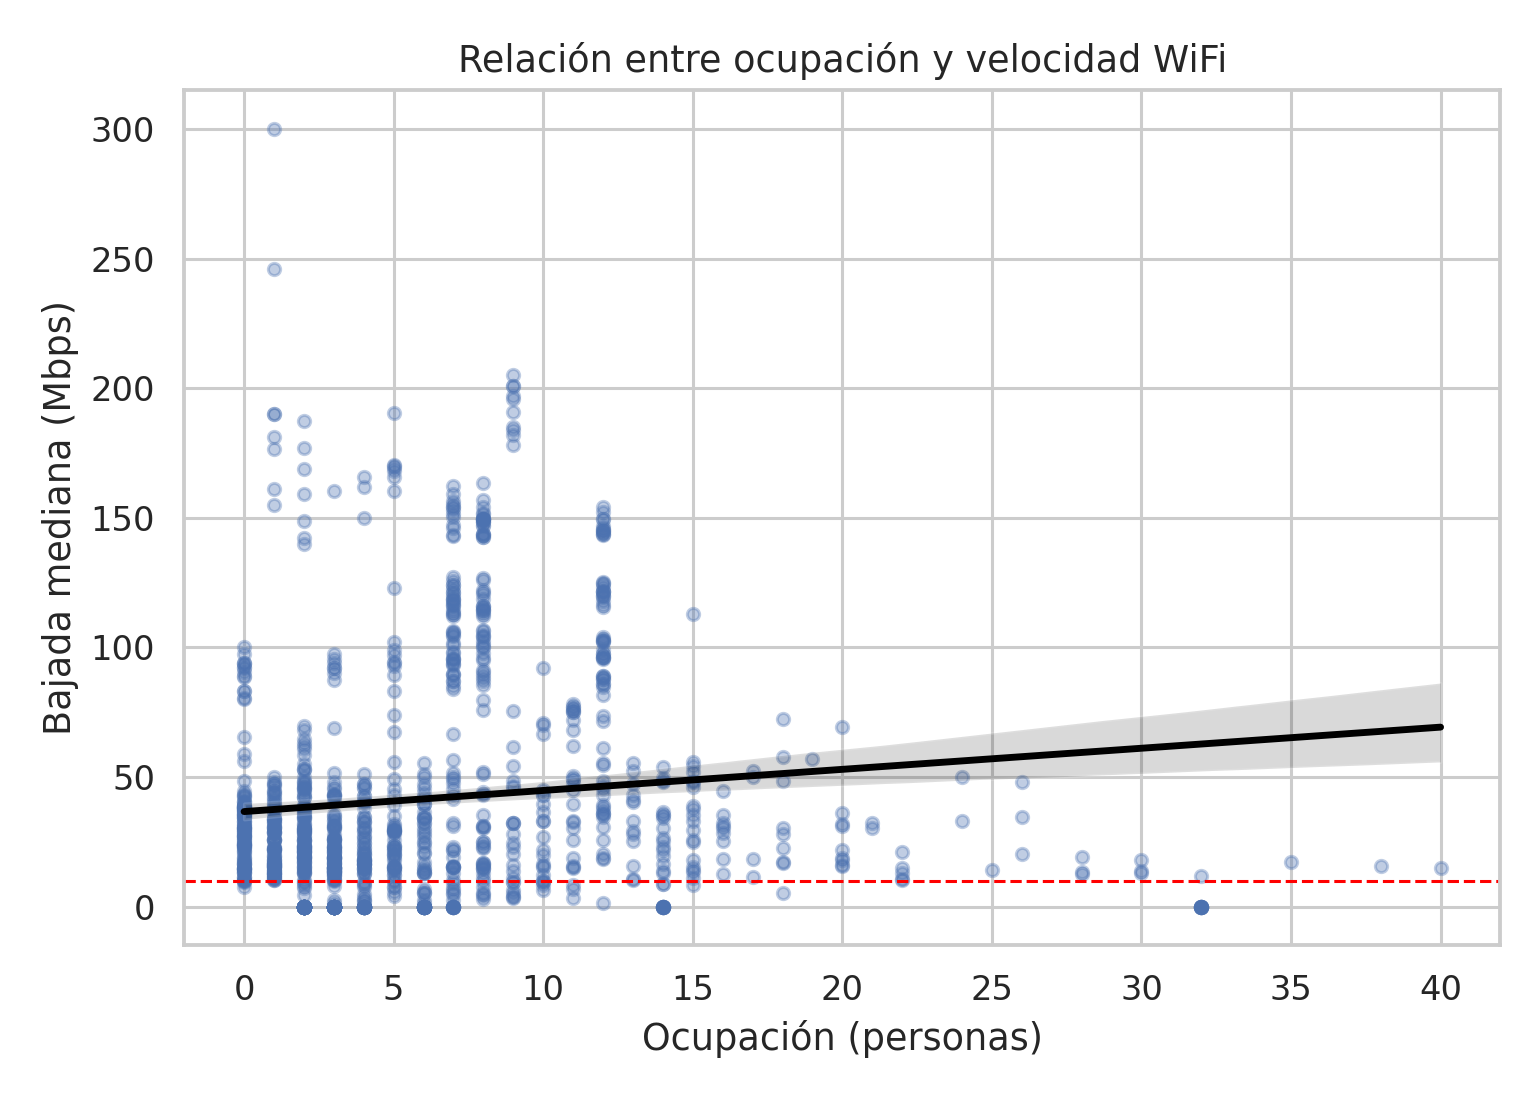
\includegraphics[width=0.8\textwidth]{figuras/scatter_ocupacion_wifi.png}
\caption{Relación entre ocupación y velocidad de bajada WiFi (ajuste lineal).}
\end{figure}
\noindent\textbf{Interpretación crítica.} La asociación más débil con WiFi sugiere que, en el periodo analizado, la red muestra resiliencia relativa frente a variaciones de aforo, aunque persisten sedes con desempeño estructuralmente bajo.

\begin{figure}[H]
\centering
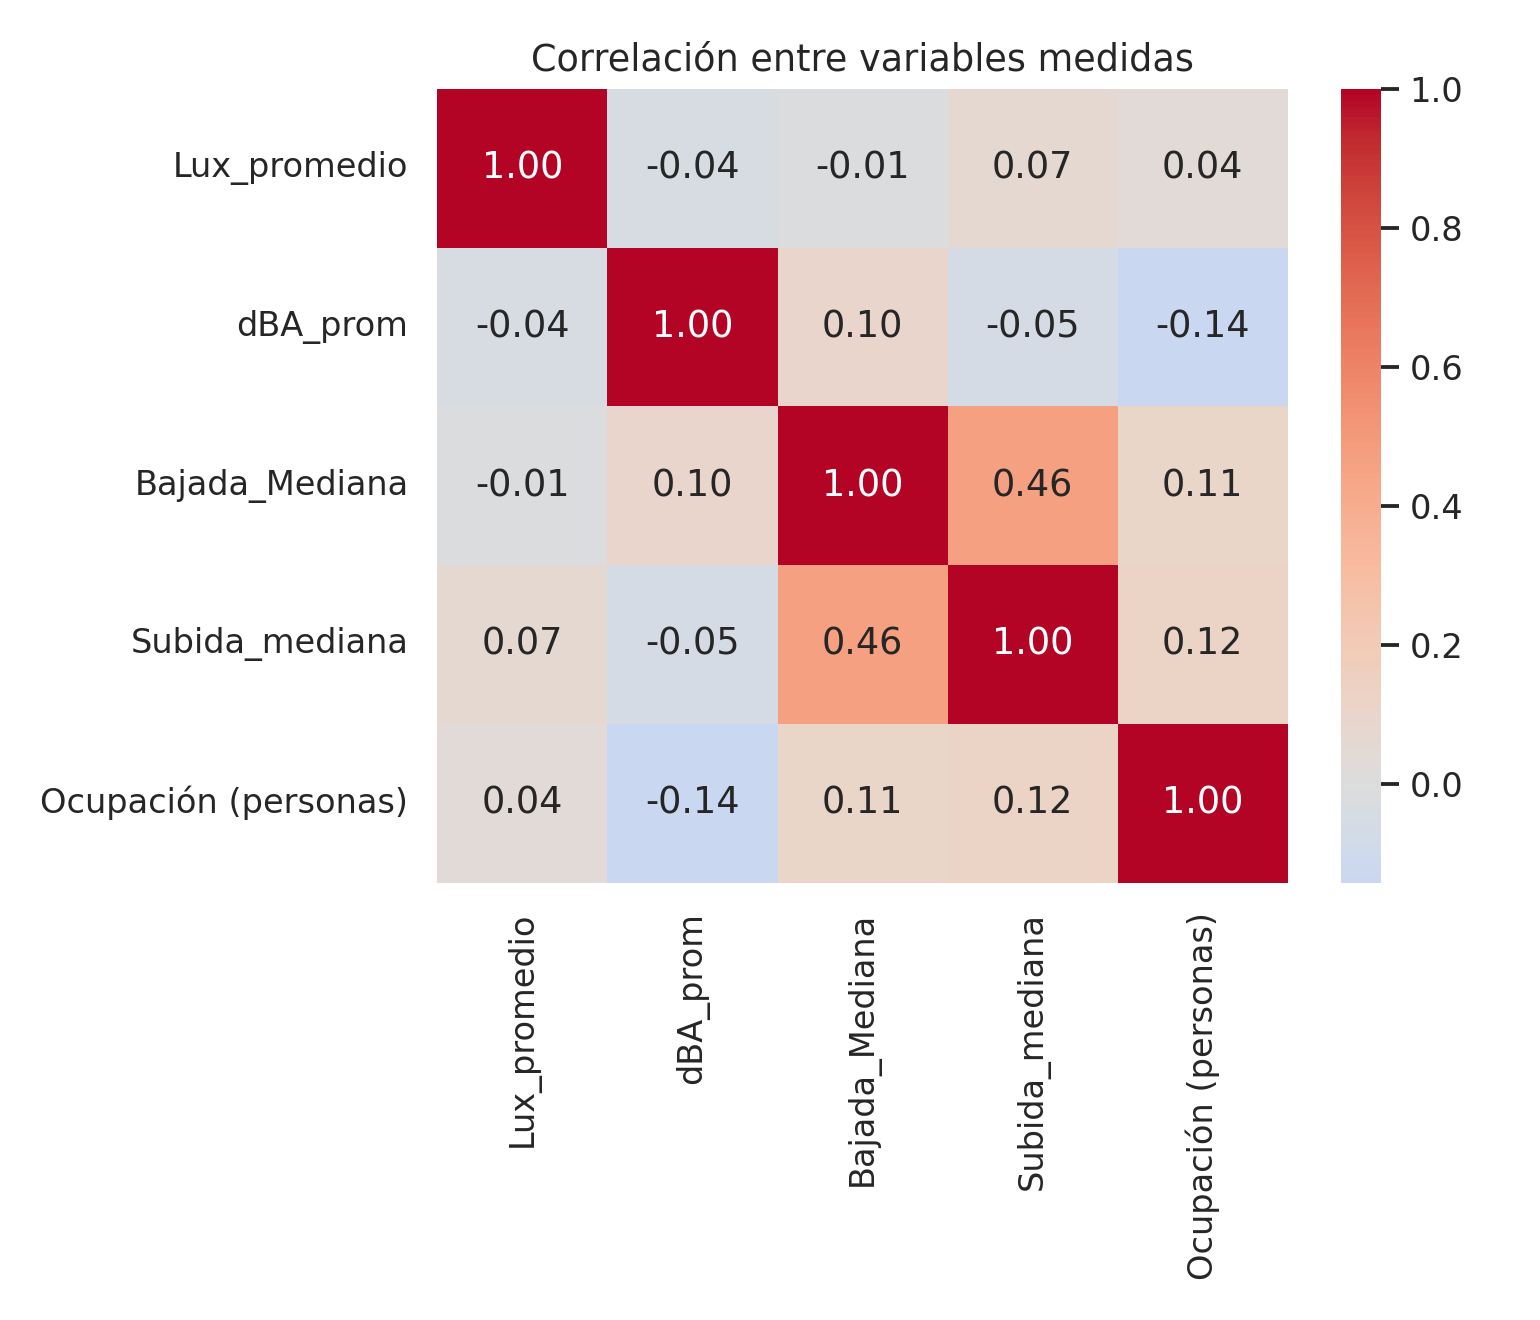
\includegraphics[width=0.80\textwidth]{figuras/correlacion_metricas.png}
\caption{Correlación entre métricas físicas y de conectividad.}
\end{figure}
\noindent\textbf{Interpretación crítica.} Las correlaciones no sustituyen causalidad, pero orientan hipótesis para diseño de intervención conjunta en infraestructura física y operación.

\begin{figure}[H]
\centering
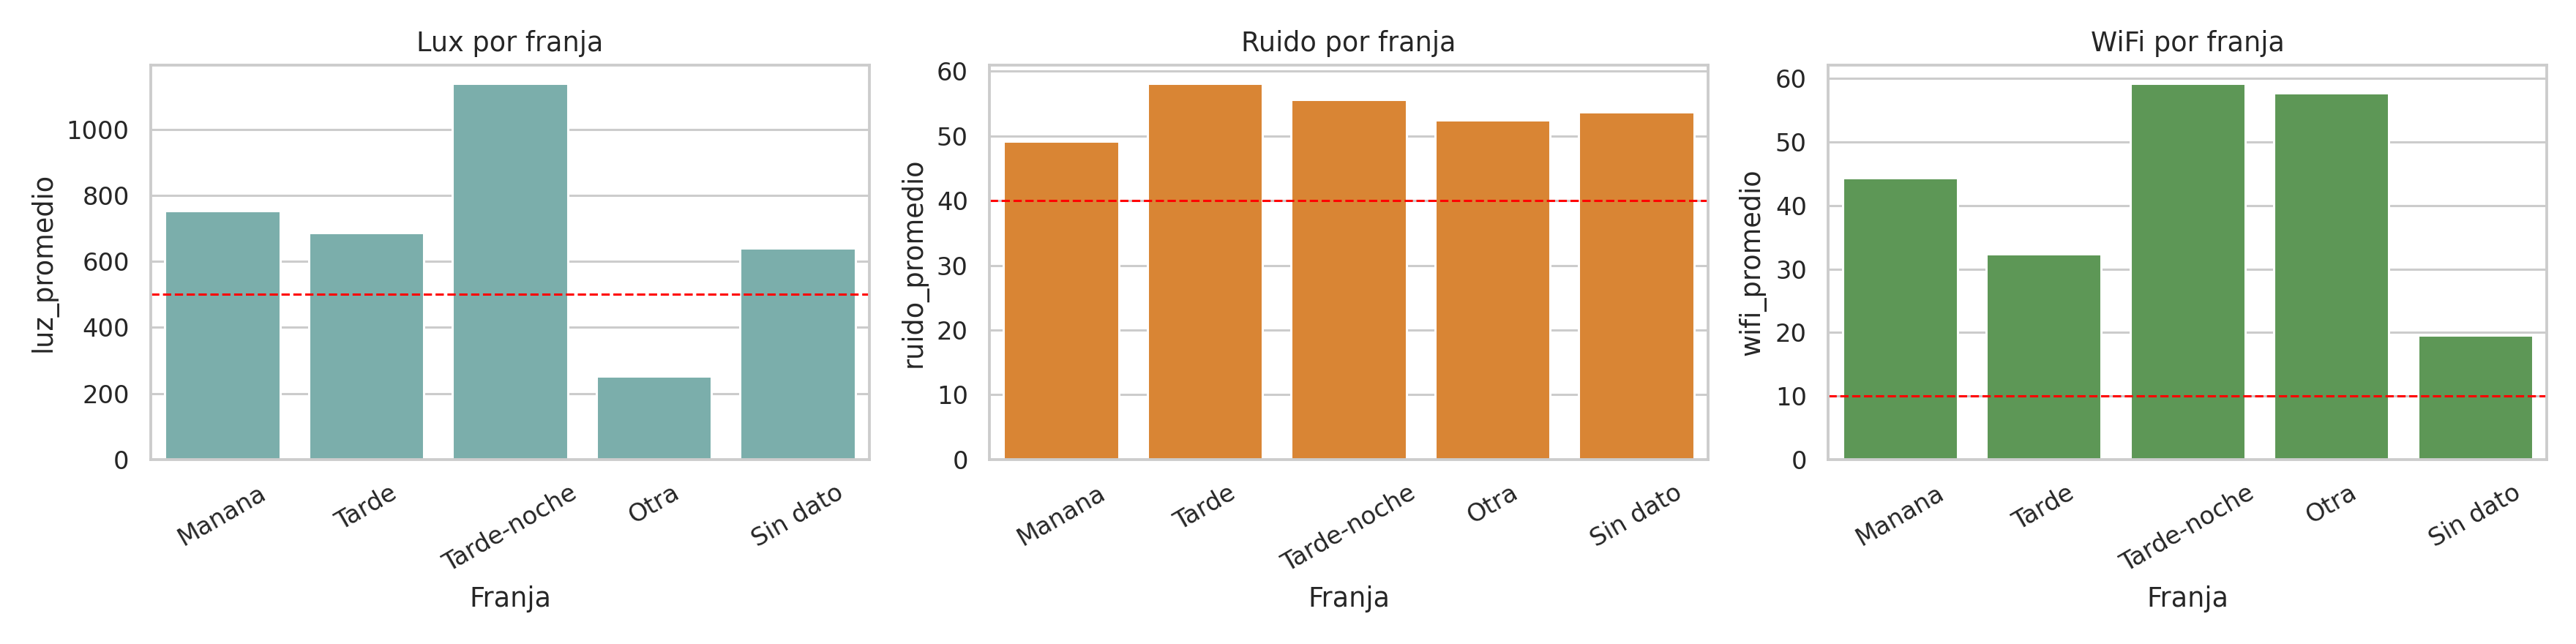
\includegraphics[width=\textwidth]{figuras/metricas_por_franja.png}
\caption{Comportamiento de métricas por franja horaria.}
\end{figure}
\noindent\textbf{Interpretación crítica.} El gradiente temporal observado permite focalizar recursos por horario, optimizando impacto de medidas de corto plazo sin esperar rediseños estructurales.

\section{Discusión}
Los resultados indican una brecha estructural entre sedes en condiciones de estudio. Esta variabilidad puede explicarse por diferencias en diseño arquitectónico, antigüedad de infraestructura, políticas de operación local, densidad de usuarios y capacidades de mantenimiento.

Desde la perspectiva de infraestructura pública urbana, los hallazgos sugieren que la calidad del servicio bibliotecario no depende solo de conectividad, sino de la interacción entre ambiente físico (ruido e iluminación), gobernanza del espacio y gestión por demanda. En contextos de alta ocupación, la calidad percibida por usuarios puede deteriorarse aun cuando la red WiFi sea aceptable.

Para política pública, esto implica migrar de un enfoque de cumplimiento mínimo a uno de desempeño integral por experiencia de usuario. En particular, el criterio acústico emerge como cuello de botella transversal, con impacto potencial sobre concentración, permanencia y rendimiento académico.


\section{Conclusiones}

\begin{itemize}
\item El sistema evaluado presenta heterogeneidad estadísticamente significativa entre bibliotecas en iluminación, ruido y conectividad; no es metodológicamente válido tratarlas como unidades equivalentes.
\item El ruido es la dimensión más crítica para el confort de estudio, con incumplimientos recurrentes y asociación positiva con ocupación.
\item La conectividad muestra mejor desempeño relativo, pero con asimetrías entre sedes y eventos atípicos que afectan continuidad de servicio.
\item El índice ponderado propuesto mejora la sensibilidad diagnóstica frente al índice simple, al reflejar mayor peso de variables de confort ambiental para actividades de lectura y estudio.
\item Se recomienda institucionalizar monitoreo periódico y tablero de control por sede, integrando indicadores de tendencia central, dispersión, cumplimiento e incidencia de outliers.
\end{itemize}


\section{Recomendaciones priorizadas}

\subsection*{Corto plazo (0--6 meses)}
\begin{itemize}
\item Implementar gestión acústica operativa: zonificación silenciosa, señalización y control de actividades ruidosas por franja.
\item Corregir puntos críticos de iluminación en áreas de lectura mediante ajustes de luminarias y mantenimiento focalizado.
\item Definir protocolo de medición mensual con alertas para incumplimientos reiterados.
\end{itemize}

\subsection*{Mediano plazo (6--18 meses)}
\begin{itemize}
\item Ejecutar intervenciones físicas de acondicionamiento acústico (materiales absorbentes, redistribución de mobiliario, barreras blandas).
\item Fortalecer arquitectura de red en sedes de mayor demanda y alta variabilidad de throughput.
\item Implementar esquema de priorización presupuestal basado en índice ponderado y tamaño de brecha.
\end{itemize}

\subsection*{Largo plazo (18+ meses)}
\begin{itemize}
\item Integrar estándares de confort ambiental y conectividad en lineamientos distritales de diseño/renovación bibliotecaria.
\item Consolidar un sistema de analítica pública longitudinal para evaluación de impacto de intervenciones.
\item Incorporar percepción de usuarios y métricas de uso académico para validar mejoras en calidad del servicio.
\end{itemize}


\section{Limitaciones y sesgos}
Entre las principales limitaciones del estudio se encuentran: (i) posibles sesgos de medición por heterogeneidad de dispositivos móviles y apps, (ii) diferencias en tamaño muestral entre bibliotecas, (iii) efecto de condiciones temporales no controladas (eventos, clima, mantenimiento puntual), y (iv) potencial dependencia intra-biblioteca por mediciones repetidas en contextos similares.

Para mitigar sesgos futuros se sugiere calibración cruzada de instrumentos, diseño de muestreo balanceado por sede y franja, y uso de modelos jerárquicos de efectos mixtos para capturar estructura anidada de los datos.


\section{Reproducibilidad}
El análisis es reproducible mediante:
\begin{itemize}
    \item Script: \texttt{scripts/analisis\_bibliotecas.py}
    \item Notebook: \texttt{Informe/Analisis\_integral\_bibliotecas\_bogota.ipynb}
\end{itemize}
La actualización del informe requiere ejecutar primero el pipeline y luego compilar este documento.

\end{document}
